\subsection{Mathematische Formeln}

\begin{frame}{\subsecname}
    Mathematische Formeln können auf verschiedene Arten und Weisen im so genannten \alert{math mode}
    gesetzt werden:
    \begin{itemize}
        \item Innerhalb von Fließtext (\alert{inline math}) mittels \code{$...$}:
            \example*{examples/inline_math.tex}
        \item Abgesetzt in einer separaten Zeile (\alert{display math}) mittels \code{[...]}:
            \example*{examples/display_math.tex}
    \end{itemize}
\end{frame}

\begin{frame}{Indizes und Exponenten}
    \begin{itemize}
        \item Indizes:
            \example*{examples/indices.tex}
            Beachte: Für Indizes mit mehr als einem Zeichen muss der Index in geschweifte Klammern
            gesetzt werden: \code{v_\{i-1\}}.
        \item Exponenten:
            \example*{examples/exponents.tex}
            Beachte: Wie bei Indizes müssen mehrere Zeichen in geschweifte Klammern gesetzt werden:
            \code{n^\{k+1\}}.
    \end{itemize}
\end{frame}

\begin{frame}{Mehrzeilige Formeln}
    \begin{itemize}
        \item Für mehrzeilige Rechnungen bieten sich Umgebungen wie \texttt{align} an:
            \example*{examples/align.tex}
        \item Die Zeilen werden dabei anhand der \code{&} ausgerichtet.
        \item Andere nützliche Umgebungen sind \texttt{equation}, \texttt{gather}, \texttt{array},
            \texttt{multiline}.
        \item Diese Umgebungen werden vom Paket \texttt{amsmath} bereitgestellt, welches daher bei
            Bedarf in der Präambel eingebunden werden muss:
            \begin{center}
                \code{\\usepackage\{amsmath\}}
            \end{center}
        \item Nummerierung kann mit \code{\\nonumber} pro Zeile ausgeschaltet werden -- oder man
            nutzt \texttt{align*} statt \texttt{align}.
    \end{itemize}
\end{frame}

\begin{frame}[t]{Mathematische Symbole}
    \begin{itemize}
        \item Das Paket \texttt{amssymb} enthält weitere mathematische Symbole:
            \begin{center}
                \code{\\usepackage\{amssymb\}}
            \end{center}
        \item Falls man einen Befehl für ein bestimmtes mathematisches Symbol sucht, hilft der Dienst
            \href{http://detexify.kirelabs.org/classify.html}{\alert{Detexify}} weiter:
            \begin{center}
                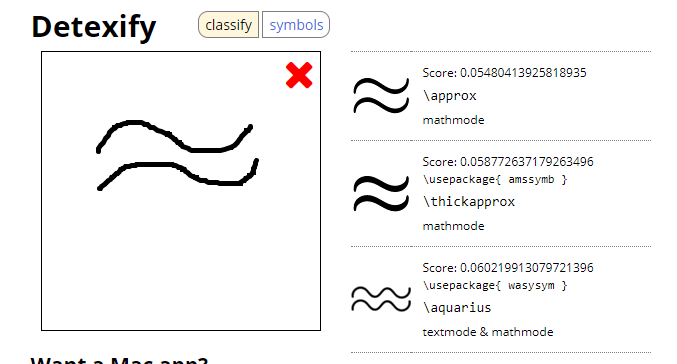
\includegraphics[keepaspectratio,width=8cm]{\thistopic/detexify.png}
            \end{center}
    \end{itemize}
\end{frame}
